\documentclass{article}

\usepackage[utf8]{inputenc}
\usepackage[russian]{babel}
\usepackage{amsmath}
\usepackage{amssymb}
\usepackage{graphicx}
\usepackage{hyperref}

\newcommand{\myparagraph}[1]{\paragraph{#1}\mbox{}\\}

\title{Homework 3}
\date{2018-29-09}
\author{Dimitrov Blagoi}

\begin{document}
  \pagenumbering{gobble}
  \maketitle
  \newpage
  \pagenumbering{arabic}

  \newpage

  \myparagraph{Задание 1}

  Пускай нам дан неотсортированный массив $x_{1}, x_{2}, x_{3}, x_{4}, x_{5}$

  Разобьем его элементы на пары и найдем в каждой из них минимум: $$(x_{1}, x_{2}) ; (x_{3}, x_{4}) ; (x_{5})$$

  НУО скажем, что $x_{1} = \min(x1, x2)$ и $x_{3} = \min(x3, x4)$.

  Также, НУО $x_{1} = \min(x1, x3)$.

  Запишем полученную нами за 3 сравнения информацию в виде бинарного дерева поиска.

  \begin{figure}[h!]
  	\centering
	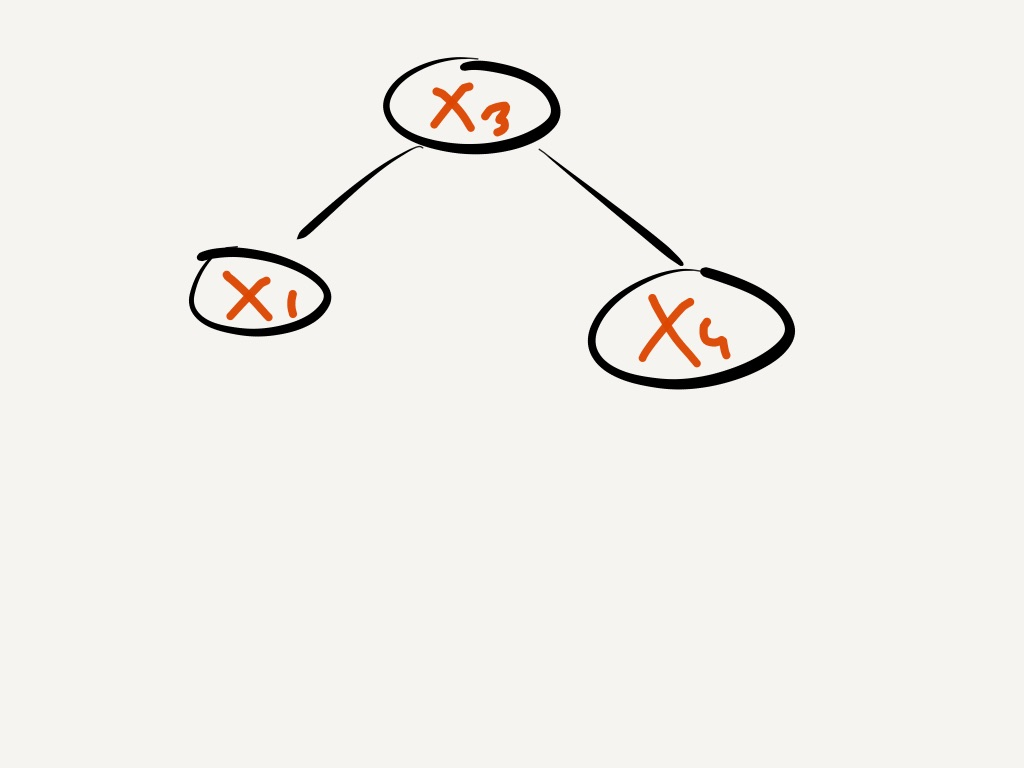
\includegraphics[width = 0.4\linewidth]{Pictures/Picture1.jpg}
  \end{figure}

  Теперь вставим в дерево $x_{5}$ за 2 сравнения. Не важно где он конкретно окажется в этом дереве, важно в какой главной ветви.

  \begin{figure}[h!]
  	\centering
  	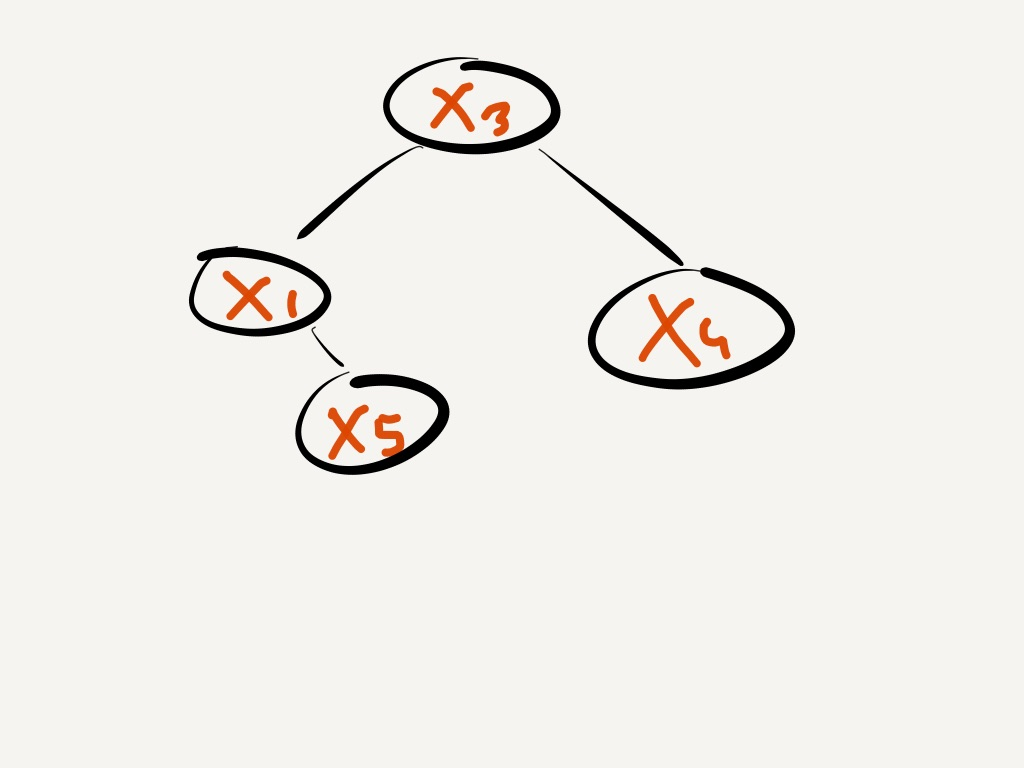
\includegraphics[width = 0.4\linewidth]{Pictures/Picture3.jpg}
	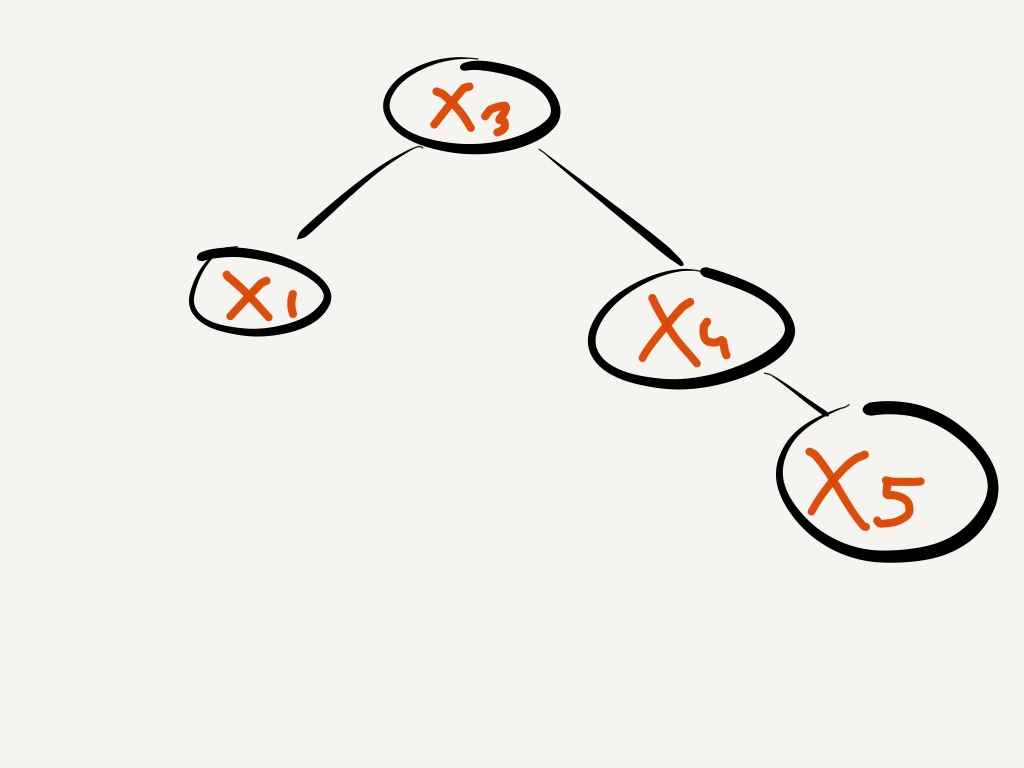
\includegraphics[width = 0.4\linewidth]{Pictures/Picture2.jpg}
  \end{figure}

  Переподвесим дерево так, чтобы элемент $x_{1}$ оказался в большей ветви дерева. В случае, показанном на левом рисунке, делать ничего не надо.

  \begin{figure}[h!]
  	\centering
  	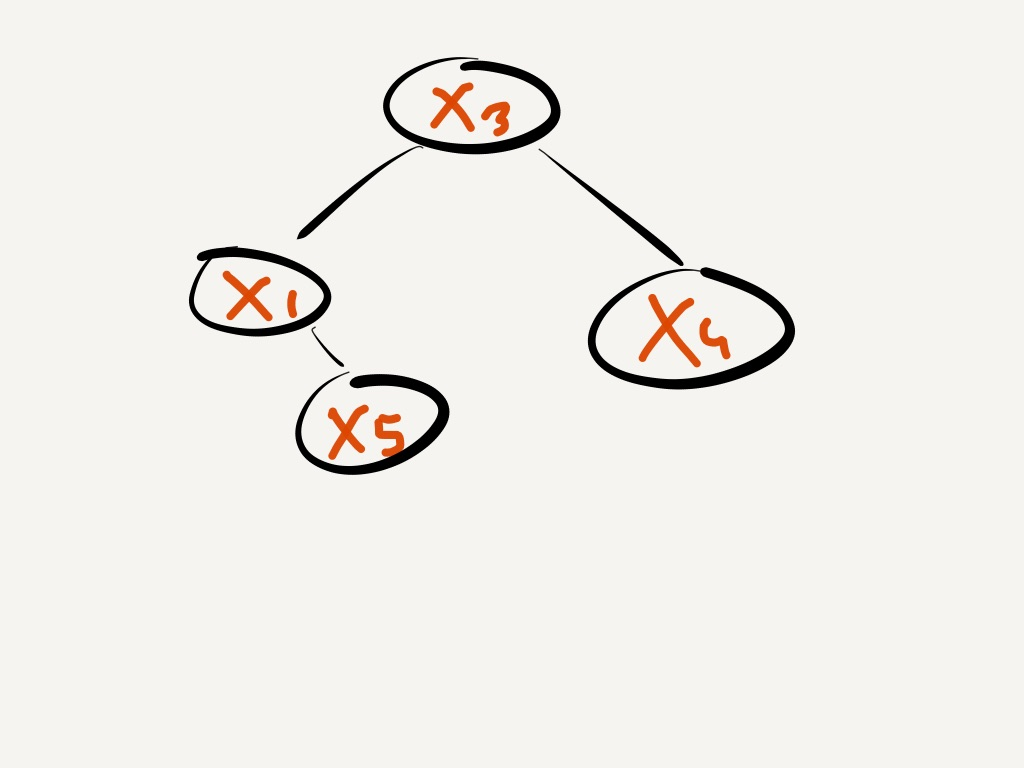
\includegraphics[width = 0.4\linewidth]{Pictures/Picture3.jpg}
	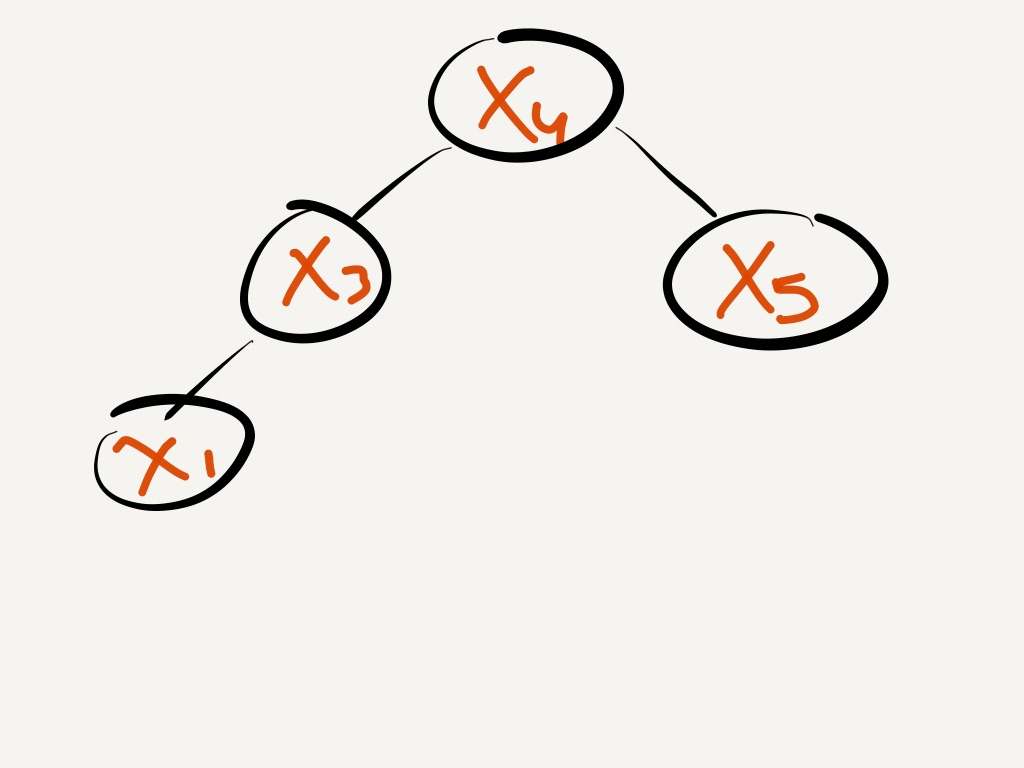
\includegraphics[width = 0.4\linewidth]{Pictures/Picture4.jpg}
  \end{figure}

  За 2 сравнения вставим в дерево элемент $x_{2}$. Почему за 2? Рассмотрим левый рисунок. Потому что мы сравним $x_{2}$ либо с $x_{3}$ и $x_{4}$, либо с $x_{3}$ и $x_{5}$ (в последнем случае сравнивать с $x_{1}$ уже не надо, т.к. мы уже сделали это ранее). Для правого рисунка - аналогично

  Итого: 7 сравнений. 

  По \href{https://www.geeksforgeeks.org/lower-bound-on-comparison-based-sorting-algorithms/}{Теореме о нижней оценке для сортировки сравнениями}, если h - высота дерева, которое можно сопоставить любому алгоритму сортировки сравнениями массива из $n$ элементов, то: 
  $$ h \geq \log_2 n! $$
  В нашем случае $h \geq \log_2 5! \approx 6,9 $, следовательно необходимо сделать как минимум 7 сравнений.

  \begin{flushright}
    $\blacksquare$
  \end{flushright}

  \myparagraph{Задание 2}

  Очевидно, что макcимальное количество перестановок при сортировке выбором массива из n элементов - $n-1$.

  Пример такой перестановки для массива из n элементов:
  $$ n, 1, 2, ..., (n - 2), (n - 1) $$
  (примечание здесь и далее: 1 - минимальный элемент, 2 - следующий по величине после минимального элемент и т.д.)

  количество таких перестановок для массивов из n элементов:$(n - 1)!$ 

  Доказательство:

  Из ответа в задании 3 (см. ниже), а также из условия задачи 4 (см. условие), напрямую следует, что так как необходимо сделать биекцию между перестановками из 2 и 3 задач, то количество перестановок в задаче 2 и 3 одинаково, то есть $(n - 1)!$

  \begin{flushright}
    $\blacksquare$
  \end{flushright}

  \myparagraph{Задание 3}

  Пример перестановки для массива из n элементов для которой требуется выполнить все $n - 1$ итерации сортировки пузырьком (в моей реализации всплывает вверх больший элемент):
  $$ n, (n - 1), ..., 2, 1 $$

  Теперь рассмотрим массив из n элементов и попробуем понять, сколько таких перестановок существует. Довольно очевидно, что, чтобы выполнялась $n - 1$ итерация алгоритма, то для всех элементов, кроме минимального, должен быть элемент, меньший по значению, но больший по индексу в начальном, неотсортированном массиве. Если такого элемента нет, то значит, что справа от него в массиве все элементы большие его, а слева меньшие, значит он стоит на своем месте, и при этом на нем и останется до конца алгоритма.

  Из этого следует, что единица(минимальный элемент) стоит на самом правом месте, ведь иначе двойка(следующий по величине после минимального элемент) должна стоять левее единицы, аналогично для трех, четырех и т.д. То есть весь массив должен уместиться слева от единицы, что невозможно, ведь она стоит не на самом правом месте.

  Если минимальный элемент стоит справа от всех, и уменьшает свой индекс не более чем на 1 за итерацию, то должно быть сделано $n-1$ итераций. Стоит отметить, что нам не важно, как расположены остальные $n - 1$ элементов, значит для массива из n элементов существует $(n - 1)!$ переставновок.

 \end{document}